% This is LLNCS.DEM the demonstration file of
% the LaTeX macro package from Springer-Verlag
% for Lecture Notes in Computer Science,
% version 2.4 for LaTeX2e as of 16. April 2010
%
\documentclass[spanish]{llncs}
%
\usepackage{pdfpages}
\usepackage{graphicx}
\usepackage[spanish]{babel}
\usepackage[utf8]{inputenc}
\usepackage{makeidx}  % allows for indexgeneration
\usepackage{url}
%
\begin{document}
%

\mainmatter              % start of the contributions
%
\title{Análisis de la herramienta TLA+ Proof System}
%
%
\author{Pablo Celayes, Giovanni Rescia, Ariel Wolfmann}

%
\institute{Facultad de Matemática, Astronomía y Física\\
Universidad Nacional de Córdoba}

\maketitle              % typeset the title of the contribution

\begin{abstract}
Agente: Cuando yo le diga hola señor Thompson, usted dice, hola

Homero: ¡Bien!

Agente: ¡¡Hola señor Thompson!!

Homero: ... ...

Agente: ¡¡Recuerde!! ¡su nombre ahora es Homero Thompson!

Homero: ¡¡Enterado!!

Agente: ¡¡Hola señor Thompson!!

Homero: (al otro agente)¡¡Creo que le habla a usted!!!. \dots

\keywords{model checking, proof system, recibirse}
\end{abstract}
%

\section{Contexto de creación de la herramienta}

 En 1977, Amir Pnueli introdujo el uso de lógica temporal para describir el comportamiento de un sistema. En principio, un sistema se podía describir con una sola fórmula de lógica temporal. En la práctica no era así. La lógica temporal de Pnueli era ideal para describir ciertas propiedades de los sistemas, pero poco adecuada para muchas otras. Es por ello que normalmente se la combinaba con maneras más tradicionales de describir sistemas. \cite{pnueli}

A fines de los 80's Leslie Lamport inventó el lenguaje TLA (Temporal Logic of Actions, una variante simple de la lógica temporal de Pnueli). TLA facilita la tarea de describir un sistema completo en una sola fórmula. La mayor parte de una especificación TLA se compone de Matemática ordinaria, no temporal. La lógica temporal sólo juega un rol significativo en la descripción de aquellas propiedades para las que realmente es buena. \cite{specsys}

En 2001, Lamport comenzó a trabajar en el centro \textit{Microsoft Research} de Mountain View, Estados Unidos. De esta etapa surge el proyecto TLA+ Proof System (TLAPS) que actualmente se desarrolla como parte del proyecto \textit{Tools for Proofs} en el centro conjunto de investigación \textit{Microsoft Research - INRIA} de Palaiseau, Francia. El proyecto cuenta con una activa lista de mail para discusiones relativas a su uso y un sistema público de seguimiento de \textit{bugs}.

% Comentar repercusiones, cómo es que termina en Microsoft y cómo se relacione esto con la evolución del Toolbox y sus aplicaciones en la industria.

% Distinguir TLA y TLA+

\section{Objetivo de la herramienta}

TLAPS es una herramienta que verifica mecánicamente la correctitud de pruebas escritas en TLA+.
Éste es un lenguaje de especificación de propósito general, orientado a sistemas concurrentes y distribuidos.

En general, una prueba de TLA+ es una colección de sentencias estructuradas jerárquicamente,
donde cada sentencia tiene una afirmación, injustificada o justificada por una colección de hechos citados.

El propósito de TLAPS es verificar las pruebas de teoremas propuestas por el usuario, es decir,
que la jerarquía de las sentencias de hecho establecen la veracidad del teorema si las afirmaciones fueran ciertas,
y luego verificar que la afirmación de cada sentencia justificada es implicada por los hechos citados.

Si un teorema de TLA+ tiene una prueba con todas sus afirmaciones justificadas, entonces, como resultado
de comprobar la prueba, TLAPS verifica que el teorema es cierto.

\section{Descripción de la herramienta del lado del usuario}

TLA+ es una herramienta de alto nivel para la descripción de los sistemas, especialmente sistemas concurrentes asíncronos y distribuidos. 
Fue diseñado para ser simple, muy expresivo, y permitir una formalización directa del razonamiento de aserciones tradicional.
Se fundamenta en la idea de que la mejor manera de describir formalmente es con matemática simple, y que un lenguaje de especificación debe contener lo menos posible más allá de lo que se necesita para escribir matemática simple con precisión.

Para cumplir con el objetivo de formalizar el razonamiento de aserciones, TLA+ está basado en TLA (\textit{Temporal Logic of Actions}), una variante simple de la lógica temporal lineal.

% itemizar esto, mencionar toolbox
TLA+ utiliza a PlusCal como lenguaje de especificación.
Para el modelado se basa en el modelo Standard.
TLC es quien se encarga de verificar la corrección de los modelos.
Finalmente, TLA+ Proof System es un asistente de pruebas, para verificar las especificaciones dadas en TLA+. 
En esta herramienta específica es donde nos enfocaremos el resto del documento. 


Cabe aclarar que TLA+ posee una interfaz gráfica donde el usuario puede utilizar todas estas herramientas de manera sencilla e integrada.

  \subsection{PlusCal}
  TLA+ utiliza PlusCal como lenguaje en el cual se debe realizar la especificación.
  PlusCal es un lenguaje algorítmico que, a primera vista, parece un lenguaje de programación imperativo pequeño. Sin embargo, una expresión PlusCal puede ser cualquier expresión de TLA+, lo que significa cualquier cosa que pueda ser expresada con matemática. Esto hace a PlusCal mucho más expresivo que cualquier lenguaje de programación.
  Un algoritmo PlusCal se traduce (compila) en una especificación TLA+, la cual puede ser chequeada con las herramientas de TLA+.
  Fue diseñado para  reemplazar al  pseudocódigo, conservando su sencillez y proporcionando al mismo tiempo un lenguaje formalmente definido y verificable, en el cual las personas sin tantos conocimientos profundos en matemática pueden definir su especificacion de forma sencilla y facil de entender,
  para luego traducirla a TLA+ usando la herramienta.

  \subsection{Modelo STANDARD}
  En un modelo \textit{Standard}, un sistema abstracto se describe como un conjunto de comportamientos, cada uno representando una posible ejecución del sistema, donde un comportamiento es una secuencia de estados y un estado es una asignación de valores a las variables.
  En este modelo, un evento, también llamado un paso, es la transición de un estado a otro en un comportamiento.

  \subsection{TLC}
  El chequeador de modelos TLC construye un modelo de estado finito de las especificaciones TLA+ para el control de las propiedades de invariancia.
  Genera un conjunto de estados iniciales que satisfacen la especificación y a continuación realiza una búsqueda en amplitud (Breadth-First Search) sobre todas las transiciones de estado definidas. 
  La ejecución se detiene cuando todas las transiciones de estado conducen a estados que ya han sido descubiertos. Si TLC descubre un estado que viola un invariante del sistema, se detiene y ofrece una traza infractora. En caso de que haya alcanzado un estado que no tenga posibles acciones habilitadas, 
  reporta un mensaje de error explicitando el posible \textit{deadlock} (opcional).
  
  TLC ofrece un método de declarar simetrías del modelo para evitar el fenómeno de \textit{explosión combinatoria}.
  También paraleliza el paso de la exploración del estado, y se puede ejecutar en modo distribuido para repartir la carga de trabajo a través de un gran número de computadoras.
  
  TLA+ es un ejemplo de lenguaje de mucha expresividad, puede ser fácilmente utilizado para especificar un programa que acepte una máquina de Turing arbitraria como entrada y puede determinar si se detendrá o no.
  Ningún chequeador de modelos puede manejar todas las especificaciones TLA+. TLC maneja un subconjunto de TLA+ que intenta incluir la mayoría de las especificaciones algorítmicas y propiedades de corrección, así como todas las especificaciones de diseño de protocolos y sistemas.

  \subsection{TLA+ Proof System}
  TLAPS, el sistema de prueba de TLA+, es una plataforma que extiende a TLA+, para el desarrollo y verificación mecánica de demostraciones. 
  
  El lenguaje de pruebas de TLA+ es declarativo y requiere cierto conocimiento previo de matemática elemental. Soporta desarrollo incremental y verifica la estructura jerárquica de la demostracion.
  
  La herramienta traduce una demostración en un conjunto de pruebas independientes, y llama a una colección de verificadores que se encargan de chequearlas, 
  que incluyen demostradores de teoremas, asistentes de pruebas, chequeadores de satisfacibilidad y procedimientos de decisión.
  
  La versión actualmente disponible TLAPS maneja casi toda la parte no temporal de TLA+, como así también el razonamiento temporal necesario para probar propiedades de seguridad (\textit{safety}) estándar, en particular invariantes y simulación de transiciones, pero no para propiedades de vitalidad (\textit{liveness}).
  
  Desarrollar demostraciones es complejo y propenso a errores, por lo que previo a verificar la correctitud de una especificación,
  se recomienda chequear instancias finitas con TLC. Esto usualmente detecta varios errores sencilla y rápidamente. 
  Una vez que TLC no encuentra errores, se puede intentar probar la correctitud de una demostración. 

  
\section{Aspectos técnicos de la herramienta}

La arquitectura general de TLAPS (Fig. 1) se divide en: el administrador de pruebas de LTA (\textit{LTAPM}) y tres \textit{backends} que éste invoca: Isabelle, Zenon y SMT (Satisfiability Modulo Theories).

\begin{figure}
  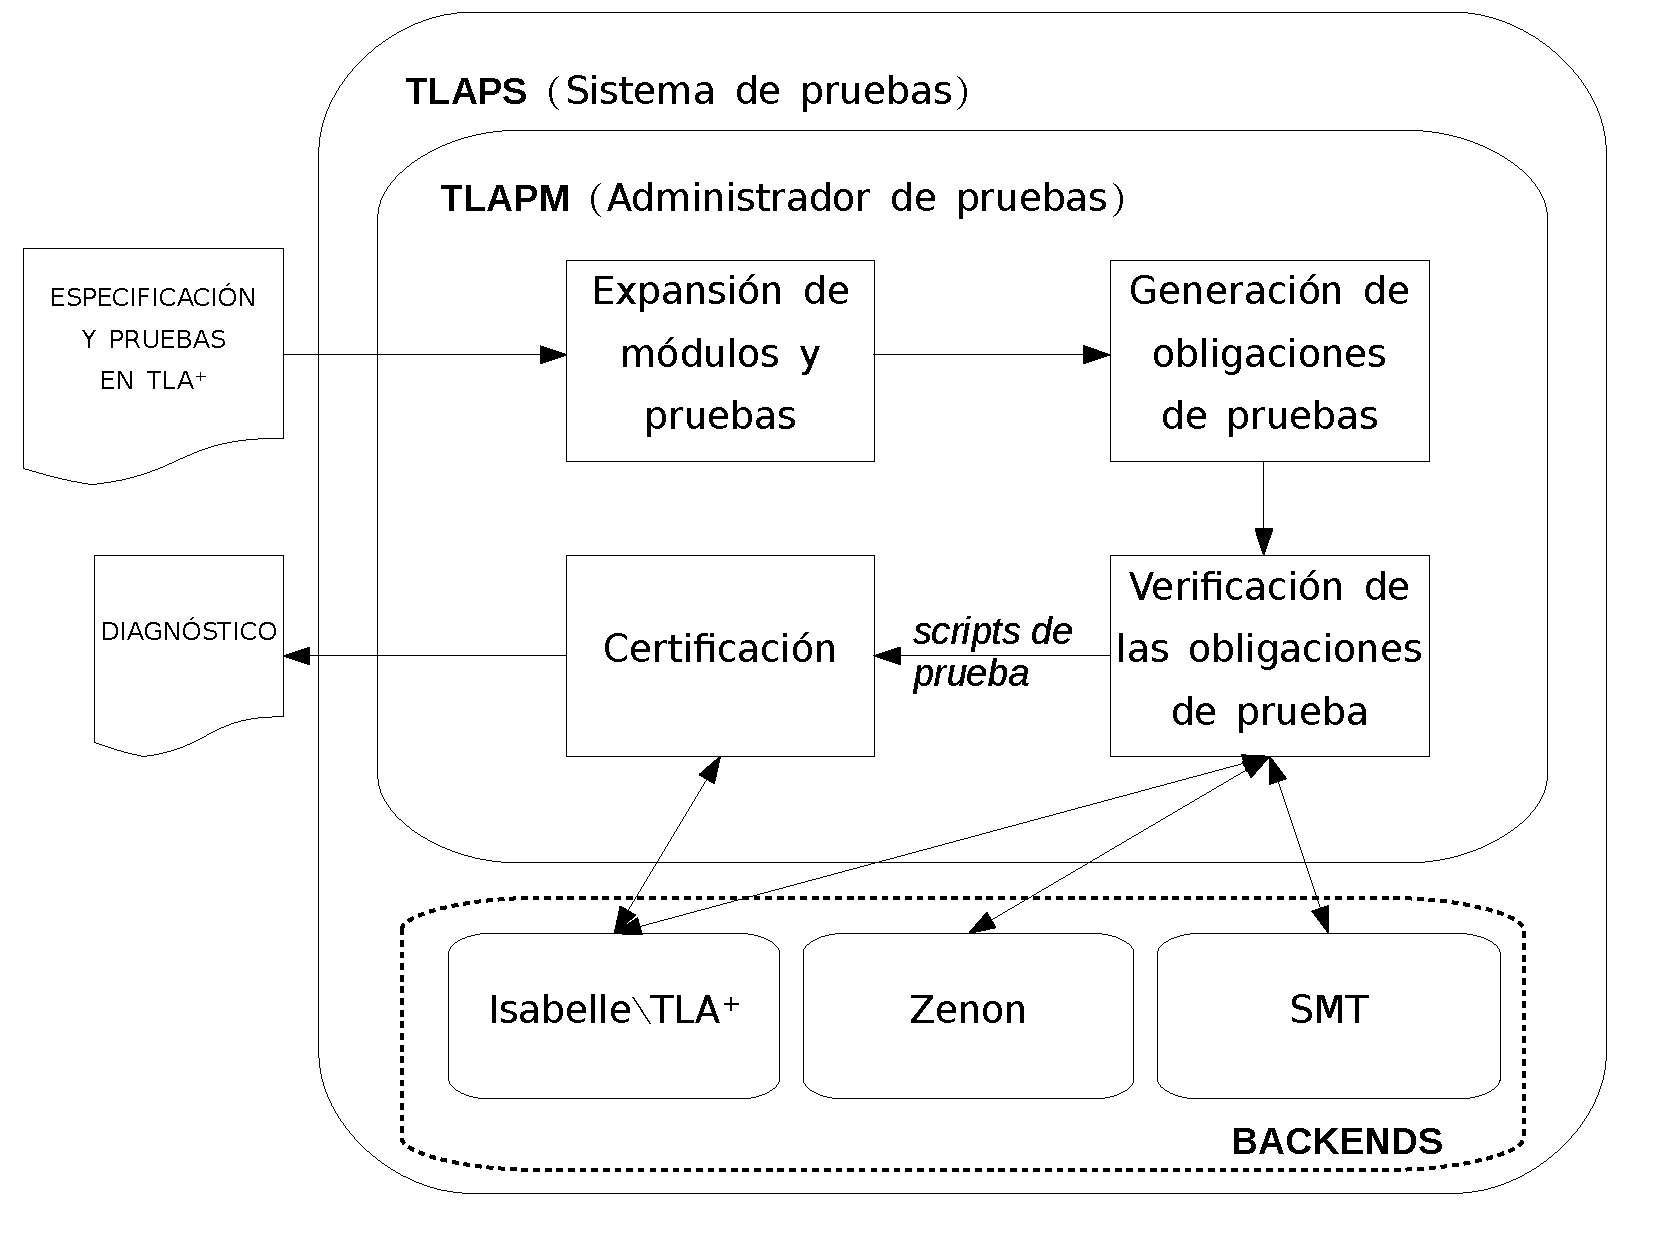
\includegraphics[scale=0.4]{esquema-informe-ingsoft2}
  \caption{Arquitectura general del entorno de pruebas TLAPS}
\end{figure}

  
  \subsection{LTAPM}
  
  Una especificación en TLA+ consiste de un módulo raíz que puede (transitivamente), importar otros módulos por extensión e instanciación con
  sus respectivos parámetros. Cada módulo consiste en:

  \begin{itemize}
   \item parámetros (variables, o estados, y constantes sin interpretar)
   \item definiciones
   \item teoremas, que pueden tener su prueba
  \end{itemize}

  Un parámetro de un módulo puede ser una variable (estado), o una constante; en las fórmulas de TLA+ no se hace referencia explícita a las variables, en cambio, se usan dos copias de una variable \textit{v}: \textit{v} y \textit{v'}, que hacen referencia a un valor antes, y después de la transición. 
  TLAPS se ejecuta invocando a TLAPM en el módulo raíz e indicando qué pruebas chequear. 

  %   ¿esto hay que sacarlo o ampliar?
  %   R: Eso es la referencia al paper del cuál saqué la info :)
  (Verifying Safety Properties With the TLA+ Proof System).
  \\
  
  El siguiente paso del LTAPM, es generar \textit{obligaciones de prueba} para cada prueba terminal, es decir, las cosas que se tienen que demostrar, o corroborar, para probar la correctitud del teorema. Una vez generadas las obligaciones de prueba, organiza la ejecución de los backends para que las verifiquen.
  \\
  
  Cada obligación de prueba es independiente y puede ser probada por separado. Cuando los backends no pueden encontrar una prueba en un límite razonable de tiempo, el sistema informará cuál obligación es la que falló, junto con su contexto (falló, cancelada por el usuario, omitida) y objetivo de la prueba.
  El usuario debe entonces determinar si falló debido a que depende de hechos o definiciones ocultas, o si el objetivo es demasiado complejo y necesita ser refinado con otro nivel de prueba. Esto indica que pueden haber obligaciones que son ciertas, y que por una cuestión de \textit{timeout},
  el backend las verifica como falsas.
  \\
  
  Si un backend encuentra una prueba de una obligación, es decir si la puede verificar, genera una traza de la prueba realizada, llamada \textit{certificación de prueba}. LTAPM  mediará la certificación de los scripts de prueba en un entorno lógico confiable, que en el diseño actual es Isabelle/TLA+.
  \\
  
  Finalmente, luego de certificar todas las obligaciones de prueba posibles generadas por las pruebas
  terminales, se procede a certificar el teorema en sí, en un proceso de dos pasos. 
  
%   chequear coherencia de esta oración:
  Primero, LTAPM genera la estructura de un lema (y sus pruebas en Isabelle/TLA+) que establece simplemente que la colección de
  obligaciones de pruebas terminales implican el teorema.
  \\
  
  Luego, LTAPM genera una prueba del teorema usando la estructura del lema y las obligaciones ya certificadas. Si Isabelle acepta la prueba, estamos seguros de que la versión traducida del teorema es verdadera en Isabelle/TLA+.

  \subsection{Backends}
  \subsection*{Zenon}
	Es el backend invocado por defecto por el TLAPM. Es un demostrador de teoremas automático para lógica clásica de primer orden (con igualdad), basado en el método tableau. Inicialmente diseñado para generar pruebas chequeables en el demostrador de teoremas Coq. Ahora extendido para generar scripts de pruebas chequeables en Isabelle. Uno de sus objetivos de diseñoo es resolver problemas simples de manera rápida.
	(Zenon: an Extensible Automated Theorem Prover Producing Checkable Proofs)
  \subsection*{Isabelle}    
	Es un demostrador de teoremas genérico, diseñado para hacer razonamiento interactivo en una variedad de teorías formales. Provee un lenguaje para describir las lógicas-objeto y para probar sus teoremas. Es invocado cuando la prueba en Zenon falla.
	(Verifying Safety Properties With the TLA+ Proof System).
  \subsection*{SMT}
	Es particularmente bueno en problemas difíciles que involucran aritmética, funciones sin interpretar y cuantificadores.
	(Formal Techniques for Distributed Systems).

\section{Casos de aplicación de la herramienta}


\subsection{Amazon}
\textit{Amazon Web Services} utiliza TLA+ desde 2011. Haciendo \textit{model checking} sobre TLA+ se han descubierto bugs
en DynamoDB, S3, EBS, y en un \textit{lock manager} interno distribuído.

Algunos bugs requirieron trazas de 35 pasos para ser detectados. También se ha usado model checking para verificar optimizaciones agresivas.

Además, las especificaciones TLA+ han resultado valiosas como documentación y ayudas de diseño.
\cite{amazon}

\subsection{XBOX 360}
Microsoft usó TLA+ para encontrar y resolver un \textit{bug} en el sistema de memoria de la consola \textit{XBOX 360}.
\cite{xbox360}


\section{Comparación con otras herramientas}
Para realizar la comparación con otras herramientas decidimos primero comparar TLA+ con otra herramienta ya conocida como Alloy,
y luego abocarnos específicamente a TLAPS.

  \subsection{TLA+}
  TLA+ y Alloy poseen un concepto de modelado similar, pero TLA+ es mucho mas expresivo que Alloy. La expresividad limitada de Alloy aparece como consecuencia del enfoque particular que toma su herramienta analizadora a la hora de realizar el análisis. Alloy es limitado a las relaciones sobre los identificadores, no tiene estructuras de datos ni recursión, esto lo hace muy eficiente para verificar modelos pequeños, pero para modelos más realistas presenta problemas. 
  
  Esta diferencia toma importancia en la práctica, ya que muchas especificaciones reales escritas en TLA+ son 
  casi imposibles de escribir en Alloy.

  \subsection{TLAPS}
  Con respecto a TLAPS específicamente, las herramientas que encontramos como comparables son Isar, Focal y Coq.
    \begin{itemize}
      \item 
      \textbf{Isar} es un lenguaje de prueba declarativo, que corre sobre Isabelle, pero tiene diferencias significativas, que llevan a un estilo de desarrollo de pruebas diferente. Por ejemplo, provee un acumulador para evitar referencias explícitas a los pasos de la prueba, lo cual es bueno para pruebas cortas, pero no tanto para demostraciones largas, que son típicas a la hora de verificar algoritmos. Además como Isabelle está diseñada para uso interactivo, los efectos de los comandos de Isar para demostraciones no son fácilmente 
      predecibles, lo que estimula pruebas lineales en lugar de hacerlas jerárquicamente. 

      \item
      El lenguaje \textbf{Focal} provee un conjunto de características funcionales y orientadas a objetos, que permiten expresar formalmente una especificación, avanzando incrementalmente, comprobando que la implementacion concuerda con la especificación y el diseño con los requerimientos. Es esencialmente un subconjunto de TLA+, que incluye el desarrollo 
      de demostraciones jerárquicamente.

      \item
      \textbf{Coq} es un sistema asistente de demostraciones formales, que provee lenguaje formal para escribir definiciones matemáticas, ejecutar algoritmos y teoremas en conjunto, con un ambiente para el desarrollo semi-interactivo de demostraciones verificadas automáticamente.

    \end{itemize}
  
  Básicamente, TLAPS realiza una integración entre las funcionalidades de  Isar y Coq, ya que utiliza Isabelle y Zenon como backends.

\section{Caso de estudio elegido}
Ilustraremos la forma en que se trabaja con TLAPS a través de un ejemplo sencillo: 
El desarrollo de una prueba de correctitud del clásico \textit{Algoritmo de Euclides} para el cálculo del \textit{máximo común divisor} entre pares de números naturales.

% Otras opciones:
\section{Conclusiones particulares}



%
% ---- Bibliography ----
%
\begin{thebibliography}{5}
%
\bibitem {pnueli}
Pnueli, Amir

The temporal logic of programs

Proceedings of the 18th IEEE Symposium on Foundation of Computer Science, 1977

\bibitem {specsys}
Lamport, Leslie

Specifying Systems: The TLA+ Language and Tools for Hardware and Software Engineers

Addison-Wesley. ISBN 0-321-14306-X, 2002

\bibitem {amazon}
Chris Newcombe, Tim Rath, Fan Zhang, Bogdan Munteanu, Marc Brooker, Michael Deardeuff 

How Amazon Web Services Uses Formal Methods

Communications of the ACM, Vol. 58 No. 4, Pages 66-73

\bibitem {xbox360}
Lamport, Leslie 

Thinking for Programmers (at 21m46s) (Grabación de charla técnica). 

\url{http://channel9.msdn.com/Events/Build/2014/3-642#time=21m46s}

San Francisco: Microsoft.

\end{thebibliography}

\clearpage

\end{document}
